\documentclass[12pt,a4paper]{article}

% ==================== 宏包 ====================
\usepackage[UTF8]{ctex}                    % 中文支持
\usepackage[margin=2.5cm]{geometry}        % 页边距
\usepackage{graphicx}                      % 图片
\graphicspath{{img/}}
\usepackage{float}                         % 图片浮动控制
\usepackage{booktabs}                      % 三线表
\usepackage{longtable}                     % 跨页长表格
\usepackage{array}                         % 表格列格式
\usepackage{listings}                      % 代码高亮
\usepackage{xcolor}                        % 颜色
\usepackage{hyperref}                      % 超链接
\usepackage{amsmath}                       % 数学公式
\usepackage{caption}                       % 图表标题
\usepackage{subcaption}                    % 子图
\usepackage{enumitem}                      % 列表控制
\usepackage{fancyhdr}                      % 页眉页脚
\usepackage{titlesec}                      % 标题格式
\usepackage{indentfirst}                   % 首行缩进

% ==================== 代码样式 ====================
\definecolor{codegreen}{rgb}{0,0.6,0}
\definecolor{codegray}{rgb}{0.5,0.5,0.5}
\definecolor{codepurple}{rgb}{0.58,0,0.82}
\definecolor{backcolour}{rgb}{0.95,0.95,0.95}
\definecolor{codeblue}{rgb}{0.0,0.0,0.8}

\lstdefinestyle{verilog}{
    language=Verilog,
    backgroundcolor=\color{backcolour},
    commentstyle=\color{codegreen},
    keywordstyle=\color{codeblue}\bfseries,
    numberstyle=\tiny\color{codegray},
    stringstyle=\color{codepurple},
    basicstyle=\ttfamily\footnotesize,
    breakatwhitespace=false,
    breaklines=true,
    captionpos=b,
    keepspaces=true,
    numbers=left,
    numbersep=5pt,
    showspaces=false,
    showstringspaces=false,
    showtabs=false,
    tabsize=4,
    frame=single,
    rulecolor=\color{codegray},
    morekeywords={wire, reg, input, output, module, endmodule, assign,
                  always, posedge, negedge, begin, end, if, else, case,
                  endcase, default, parameter, include, define, timescale,
                  initial, forever},
    literate={`}{\textasciigrave}1,
}

\lstdefinestyle{mips}{
    backgroundcolor=\color{backcolour},
    commentstyle=\color{codegreen},
    keywordstyle=\color{codeblue}\bfseries,
    numberstyle=\tiny\color{codegray},
    basicstyle=\ttfamily\footnotesize,
    breaklines=true,
    captionpos=b,
    numbers=left,
    numbersep=5pt,
    frame=single,
    rulecolor=\color{codegray},
    morekeywords={add, addi, addiu, addu, sub, subu, and, andi, or, ori,
                  xor, xori, nor, sll, sllv, srl, srlv, sra, srav, lui,
                  slt, slti, sltu, sltiu, beq, bne, bgez, bgtz, blez, bltz,
                  bgezal, bltzal, j, jal, jr, jalr, lb, lbu, lh, lhu, lw,
                  lwl, lwr, ll, sb, sh, sw, swl, swr, sc, mult, multu, mul,
                  div, divu, mfhi, mflo, mthi, mtlo, madd, maddu, msub,
                  msubu, movn, movz, clz, clo, syscall, break, eret, mfc0,
                  mtc0, teq, teqi, tge, tgei, tgeiu, tgeu, tlt, tlti,
                  tltiu, tltu, tne, tnei, nop},
}

\lstset{style=verilog}

% ==================== 页眉页脚 ====================
\pagestyle{fancy}
\fancyhf{}
\fancyhead[L]{\small 计算机系统实验}
\fancyhead[R]{\small 实验一：CPU改造实验}
\fancyfoot[C]{\thepage}
\renewcommand{\headrulewidth}{0.4pt}

% ==================== 超链接样式 ====================
\hypersetup{
    colorlinks=true,
    linkcolor=black,
    citecolor=black,
    urlcolor=blue,
}

% ==================== 段落设置 ====================
\setlength{\parindent}{2em}
\setlength{\parskip}{0.5em}

% ==================== 正文 ====================
\begin{document}

% -------------------- 封面 --------------------
\begin{titlepage}
    \centering
    \vspace*{2cm}

    {\LARGE\bfseries 计算机系统实验报告 \par}
    \vspace{1.5cm}
    {\Large\bfseries 实验一：CPU改造实验 \par}
    \vspace{3cm}

    \begin{tabular}{rl}
        \textbf{姓\qquad 名：} & 韦畅 \\[8pt]    
        \textbf{学\qquad 号：} & 2352628 \\[8pt] 
        \textbf{指导教师：} & 郭玉臣 \\[8pt]     
        \textbf{实验日期：} & 2026年4月9日 \\[8pt] 
    \end{tabular}

    \vfill
    {\large 同济大学 \ 计算机科学与工程学院 \par}
    \vspace{0.5cm}
\end{titlepage}


\newpage
\tableofcontents
\newpage

% -------------------- 各章节 --------------------
\section{实验目的}

\begin{enumerate}[leftmargin=2em]
    \item 深入理解MIPS指令集体系结构，掌握五级流水线CPU的工作原理。
    \item 在已有的支持54条指令的OpenMIPS流水线CPU基础上，将其改造为支持89条MIPS指令的完整CPU。
    \item 新增指令包括：乘累加/乘累减指令（madd、maddu、msub、msubu）、除法指令（div、divu）、分支跳转指令（bgez、bgtz、blez、bltz、bltzal、bgezal、jalr）、访存指令（sb、lb、lbu、sh、lh、lhu、lwl、lwr、swl、swr、ll、sc）、移动指令（movn、movz）、算术指令（clz、clo、sltu、sllv、srav、srlv、sra、srl、subu、addu、slt等）、CP0协处理器指令（mfc0、mtc0、syscall、break、eret）、自陷指令（teq、tge、tgeu、tlt、tltu、tne及其立即数形式）。
    \item 实现CP0协处理器中的Count、Compare、Status、Cause、EPC等寄存器功能。
    \item 实现时钟中断机制。
    \item 将设计下载到Nexys DDR（Artix-7）FPGA开发板上进行验证。
\end{enumerate}

\section{实验环境}

\begin{table}[H]
    \centering
    \caption{实验环境配置}
    \begin{tabular}{ll}
        \toprule
        \textbf{项目} & \textbf{配置} \\
        \midrule
        操作系统 & Windows 11 \\
        开发工具 & Xilinx Vivado 2024.2 \\  
        汇编工具 & MARS 4.5（MIPS Assembler and Runtime Simulator） \\
        FPGA开发板 & Digilent Nexys A7（Nexys DDR） \\
        FPGA芯片 & Xilinx Artix-7 xc7a100tcsg324-1 \\
        硬件描述语言 & Verilog HDL \\
        \bottomrule
    \end{tabular}
\end{table}

\section{CPU整体架构}

\subsection{五级流水线结构}

本实验基于OpenMIPS处理器设计，采用经典的五级流水线架构：

\begin{enumerate}[leftmargin=2em]
    \item \textbf{IF（取指）阶段}：由\texttt{pc\_reg}模块根据当前PC值从指令存储器中取出指令。支持顺序取指、分支跳转和异常跳转三种PC更新方式。
    \item \textbf{ID（译码）阶段}：由\texttt{id}模块对指令进行解码，确定ALU操作类型、操作数来源、目标寄存器等。同时实现数据前推（forwarding）和load-use冒险检测。
    \item \textbf{EX（执行）阶段}：由\texttt{ex}模块执行具体的运算操作，包括逻辑运算、移位运算、算术运算、乘法运算、HI/LO寄存器操作、CP0寄存器读写和自陷指令判断。
    \item \textbf{MEM（访存）阶段}：由\texttt{mem}模块完成load/store指令的数据存储器访问，同时处理异常检测与异常类型的最终确定。
    \item \textbf{WB（写回）阶段}：将执行结果写回通用寄存器堆或HI/LO寄存器。
\end{enumerate}

流水线各级之间通过流水线寄存器（\texttt{if\_id}、\texttt{id\_ex}、\texttt{ex\_mem}、\texttt{mem\_wb}）进行数据传递，所有流水线寄存器均支持流水线暂停（stall）和流水线清空（flush）功能。

\subsection{系统顶层结构}

整个系统自顶向下分为三个层次：

\begin{itemize}[leftmargin=2em]
    \item \textbf{板级顶层}（\texttt{openmips\_board}）：负责时钟分频、数码管显示控制和显示内容选择。包含两个分频器（分别用于数码管扫描和CPU时钟），一个七段数码管驱动模块，以及SoC顶层模块。
    \item \textbf{SoC顶层}（\texttt{openmips\_min\_sopc}）：连接CPU核心、指令ROM和数据RAM，构成最小片上系统。
    \item \textbf{CPU核心}（\texttt{openmips}）：包含五级流水线的全部模块以及辅助模块（HI/LO寄存器、除法器、LLbit寄存器、CP0协处理器、流水线控制器）。
\end{itemize}

\subsection{模块列表}

\begin{table}[H]
    \centering
    \caption{设计模块一览}
    \begin{tabular}{lll}
        \toprule
        \textbf{模块名} & \textbf{功能} & \textbf{所属层次} \\
        \midrule
        \texttt{openmips\_board} & 板级顶层，时钟分频与数码管 & 顶层 \\
        \texttt{seg7x16} & 8位七段数码管扫描驱动 & 顶层 \\
        \texttt{divider} & 参数化时钟分频器 & 顶层 \\
        \texttt{openmips\_min\_sopc} & SoC顶层，连接CPU与存储器 & SoC层 \\
        \texttt{inst\_rom\_for\_cpu89} & 指令ROM（IP核） & SoC层 \\
        \texttt{data\_ram} & 数据RAM（4字节bank） & SoC层 \\
        \texttt{openmips} & CPU核心顶层 & CPU层 \\
        \texttt{pc\_reg} & PC寄存器 & IF \\
        \texttt{if\_id} & IF/ID流水线寄存器 & IF$\to$ID \\
        \texttt{id} & 译码模块 & ID \\
        \texttt{regfile} & 通用寄存器堆（32$\times$32位） & ID \\
        \texttt{id\_ex} & ID/EX流水线寄存器 & ID$\to$EX \\
        \texttt{ex} & 执行模块 & EX \\
        \texttt{ex\_mem} & EX/MEM流水线寄存器 & EX$\to$MEM \\
        \texttt{mem} & 访存模块 & MEM \\
        \texttt{mem\_wb} & MEM/WB流水线寄存器 & MEM$\to$WB \\
        \texttt{hilo\_reg} & HI/LO乘除法结果寄存器 & 辅助 \\
        \texttt{div} & 试商法除法器 & 辅助 \\
        \texttt{LLbit\_reg} & 原子操作标志寄存器 & 辅助 \\
        \texttt{cp0\_reg} & CP0协处理器寄存器 & 辅助 \\
        \texttt{ctrl} & 流水线控制与异常处理 & 控制 \\
        \bottomrule
    \end{tabular}
\end{table}

\subsection{关键设计参数}

\begin{table}[H]
    \centering
    \caption{关键设计参数}
    \begin{tabular}{ll}
        \toprule
        \textbf{参数} & \textbf{值} \\
        \midrule
        字节序 & 大端模式（Big-Endian） \\
        指令存储器起始地址 & \texttt{0x00400000} \\
        数据存储器起始地址 & \texttt{0x10010000} \\
        异常处理入口地址 & \texttt{0x00400004} \\
        指令ROM容量 & 2048 $\times$ 32位（8 KB） \\
        数据RAM容量 & 512 $\times$ 32位（2 KB） \\
        通用寄存器数量 & 32个（32位） \\
        板载时钟频率 & 100 MHz \\
        CPU工作时钟 & 经分频后约500 Hz \\
        \bottomrule
    \end{tabular}
\end{table}

\section{指令集设计}

\subsection{指令分类概述}

本CPU共支持89条MIPS指令，按功能分为以下几类：

\begin{table}[H]
    \centering
    \caption{指令分类汇总}
    \begin{tabular}{llc}
        \toprule
        \textbf{类别} & \textbf{指令} & \textbf{数量} \\
        \midrule
        逻辑运算 & and, andi, or, ori, xor, xori, nor, lui & 8 \\
        移位运算 & sll, sllv, srl, srlv, sra, srav & 6 \\
        移动操作 & mfhi, mflo, mthi, mtlo, movn, movz & 6 \\
        算术运算 & add, addi, addiu, addu, sub, subu, slt, slti, sltu, sltiu, clz, clo & 12 \\
        乘法运算 & mul, mult, multu, madd, maddu, msub, msubu & 7 \\
        除法运算 & div, divu & 2 \\
        分支跳转 & j, jal, jr, jalr, beq, bne, bgez, bgezal, bgtz, blez, bltz, bltzal & 12 \\
        加载指令 & lb, lbu, lh, lhu, lw, lwl, lwr, ll & 8 \\
        存储指令 & sb, sh, sw, swl, swr, sc & 6 \\
        CP0指令 & mfc0, mtc0, syscall, break, eret & 5 \\
        自陷指令 & teq, teqi, tge, tgei, tgeiu, tgeu, tlt, tlti, tltiu, tltu, tne, tnei & 12 \\
        空操作 & nop, ssnop, sync, pref & 4 \\
        \midrule
        \textbf{合计} & & \textbf{88+} \\
        \bottomrule
    \end{tabular}
\end{table}

\subsection{指令编码格式}

MIPS指令采用固定32位编码，共有三种基本格式：

\subsubsection{R型指令}

\begin{table}[H]
    \centering
    \begin{tabular}{|c|c|c|c|c|c|}
        \hline
        op [31:26] & rs [25:21] & rt [20:16] & rd [15:11] & sa [10:6] & func [5:0] \\
        \hline
        6位 & 5位 & 5位 & 5位 & 5位 & 6位 \\
        \hline
    \end{tabular}
    \caption{R型指令格式}
\end{table}

适用于：and, or, xor, nor, sll, srl, sra, sllv, srlv, srav, add, addu, sub, subu, slt, sltu, mult, multu, div, divu, mfhi, mflo, mthi, mtlo, movn, movz, jr, jalr, syscall, break, 自陷指令等。

\subsubsection{I型指令}

\begin{table}[H]
    \centering
    \begin{tabular}{|c|c|c|c|}
        \hline
        op [31:26] & rs [25:21] & rt [20:16] & immediate [15:0] \\
        \hline
        6位 & 5位 & 5位 & 16位 \\
        \hline
    \end{tabular}
    \caption{I型指令格式}
\end{table}

适用于：addi, addiu, andi, ori, xori, slti, sltiu, lui, beq, bne, bgtz, blez, lb, lbu, lh, lhu, lw, lwl, lwr, ll, sb, sh, sw, swl, swr, sc 等。REGIMM 类分支指令（bgez, bltz, bgezal, bltzal）及自陷立即数指令也使用此格式。

\subsubsection{J型指令}

\begin{table}[H]
    \centering
    \begin{tabular}{|c|c|}
        \hline
        op [31:26] & address [25:0] \\
        \hline
        6位 & 26位 \\
        \hline
    \end{tabular}
    \caption{J型指令格式}
\end{table}

适用于：j, jal。跳转目标地址由 PC 高4位与指令中26位地址左移2位拼接而成。

\section{核心模块设计}

\subsection{取指模块（pc\_reg）}

PC寄存器模块负责产生指令存储器的访问地址。在每个时钟上升沿，PC值按以下优先级更新：

\begin{enumerate}[leftmargin=2em]
    \item 若 \texttt{flush} 有效，PC更新为异常处理入口地址 \texttt{new\_pc}；
    \item 若流水线未暂停且分支标志有效，PC更新为分支目标地址；
    \item 否则，PC自增4（\texttt{pc + 4}）。
\end{enumerate}

复位时PC初始化为 \texttt{0x00400000}（\texttt{TextBegin}），即指令存储器的起始地址。

\begin{lstlisting}[caption={pc\_reg模块核心逻辑}]
always @ (posedge clk) begin
    if (ce == `ChipDisable)
        pc <= `TextBegin;
    else if (flush == 1'b1)
        pc <= new_pc;
    else if (stall[0] == `NoStop)
        if (branch_flag_i == `Branch)
            pc <= branch_target_address_i;
        else
            pc <= pc + 4'h4;
end
\end{lstlisting}

\subsection{译码模块（id）}

译码模块是设计中最复杂的模块之一，负责以下功能：

\begin{itemize}[leftmargin=2em]
    \item \textbf{指令解码}：根据操作码（op）、功能码（func）等字段，确定ALU操作类型（\texttt{aluop\_o}）、ALU结果选择（\texttt{alusel\_o}）、源操作数来源和目标寄存器。
    \item \textbf{数据前推}：从EX和MEM阶段获取尚未写回的计算结果，解决数据冒险。
    \item \textbf{Load-use冒险检测}：当前一条指令是load且其目标寄存器与当前指令的源寄存器相同时，插入一个流水线气泡（stall）。
    \item \textbf{分支判断}：对分支指令进行条件判断，计算分支目标地址。
    \item \textbf{延迟槽处理}：设置 \texttt{next\_inst\_in\_delayslot\_o} 标志。
    \item \textbf{异常初步检测}：识别syscall和eret指令，标记无效指令。
\end{itemize}

指令解码按操作码分为以下几类处理：

\begin{itemize}[leftmargin=2em]
    \item \texttt{op = 6'b000000}（SPECIAL类）：根据 \texttt{func} 字段区分具体指令，包含大部分R型运算指令和自陷指令。
    \item \texttt{op = 6'b000001}（REGIMM类）：根据 \texttt{rt} 字段区分 bgez/bltz/bgezal/bltzal 及自陷立即数指令。
    \item \texttt{op = 6'b011100}（SPECIAL2类）：clz、clo、mul、madd、maddu、msub、msubu。
    \item 其他I型/J型指令：根据 \texttt{op} 字段直接解码。
    \item CP0指令：通过 \texttt{inst\_i[31:21]} 特定编码识别mfc0、mtc0和eret。
\end{itemize}

\subsection{执行模块（ex）}

执行模块完成各类运算操作，内部按运算类型分为多个功能单元：

\begin{itemize}[leftmargin=2em]
    \item \textbf{逻辑运算单元}：执行 AND、OR、XOR、NOR 运算。
    \item \textbf{移位运算单元}：执行逻辑左移（SLL）、逻辑右移（SRL）、算术右移（SRA）。
    \item \textbf{算术运算单元}：执行加减法（含溢出检测）、比较运算（SLT/SLTU）、前导零/一计数（CLZ/CLO）。
    \item \textbf{乘法运算单元}：执行有符号/无符号乘法，支持乘累加/乘累减（MADD/MSUB系列），通过两周期流水线暂停实现。
    \item \textbf{除法控制}：向除法器模块发出启动信号，等待除法器完成后读取结果。
    \item \textbf{移动操作单元}：处理MFHI、MFLO、MOVN、MOVZ以及MFC0指令，包含CP0数据前推。
    \item \textbf{自陷判断单元}：判断自陷条件（相等、大于等于、小于、不等），设置 \texttt{trapassert} 信号。
    \item \textbf{CP0写控制}：处理MTC0指令，将数据写入CP0寄存器。
\end{itemize}

最终结果通过 \texttt{alusel\_i} 选择器从各功能单元中选出。同时计算访存地址 \texttt{mem\_addr\_o = reg1\_i + sign\_ext(imm16)} 供MEM阶段使用。

\subsection{访存模块（mem）}

访存模块处理所有load/store指令，实现大端模式下的字节/半字/字访问：

\begin{itemize}[leftmargin=2em]
    \item \textbf{字节访问}（LB/LBU/SB）：根据地址低2位选择4个字节bank中的对应字节，LB做符号扩展，LBU做零扩展。
    \item \textbf{半字访问}（LH/LHU/SH）：根据地址低2位选择高/低半字，LH做符号扩展。
    \item \textbf{字访问}（LW/SW）：直接读写整个32位字。
    \item \textbf{非对齐访问}（LWL/LWR/SWL/SWR）：通过拼接实现非对齐的字加载/存储。
    \item \textbf{原子操作}（LL/SC）：LL设置LLbit为1并加载数据，SC在LLbit为1时写入数据并返回1，否则返回0。
\end{itemize}

访存模块还负责异常的最终判定。它综合考虑中断、syscall、无效指令、自陷、溢出和eret等异常类型，根据CP0的Status和Cause寄存器确定是否真正触发异常，并输出最终的异常类型码。异常发生时，通过 \texttt{mem\_we\_o} 的屏蔽机制确保异常指令不会修改存储器。

\subsection{CP0协处理器（cp0\_reg）}

CP0协处理器模块实现了以下寄存器：

\begin{table}[H]
    \centering
    \caption{CP0寄存器}
    \begin{tabular}{llll}
        \toprule
        \textbf{编号} & \textbf{名称} & \textbf{读写} & \textbf{功能} \\
        \midrule
        9 & Count & 可读写 & 计数器，每个时钟周期自增1 \\
        11 & Compare & 可读写 & 比较值，当Count等于Compare时触发时钟中断 \\
        12 & Status & 可读写 & 状态寄存器，控制中断使能和异常级别 \\
        13 & Cause & 部分可写 & 原因寄存器，记录异常原因码 \\
        14 & EPC & 可读写 & 异常返回地址 \\
        15 & PRId & 只读 & 处理器标识 \\
        16 & Config & 只读 & 配置信息（大端模式） \\
        \bottomrule
    \end{tabular}
\end{table}

\textbf{时钟中断机制}：Count寄存器每周期加1，当Count等于Compare且Compare不为0时，\texttt{timer\_int\_o}置1，向CPU发出时钟中断请求。写入Compare寄存器时自动清除中断。

\textbf{异常处理流程}：当异常发生时，CP0保存当前PC到EPC（延迟槽指令则保存PC-4），将异常原因写入Cause寄存器，并将Status[EXL]置1禁止新的异常。eret指令将Status[EXL]清0恢复正常执行。

\subsection{流水线控制模块（ctrl）}

控制模块统一管理流水线暂停和异常刷新：

\begin{itemize}[leftmargin=2em]
    \item \textbf{异常刷新}（最高优先级）：当MEM阶段检测到异常时，\texttt{flush}置1，清空整条流水线，PC跳转到异常入口地址 \texttt{0x00400004}（eret则跳转到EPC）。
    \item \textbf{EX阶段暂停请求}：由除法器或乘累加/减指令引起，暂停IF、ID、EX阶段（\texttt{stall = 6'b001111}）。
    \item \textbf{ID阶段暂停请求}：由load-use冒险引起，暂停IF和ID阶段（\texttt{stall = 6'b000111}）。
\end{itemize}

\subsection{数据存储器（data\_ram）}

数据RAM采用4个独立字节bank（\texttt{data\_mem0\textasciitilde 3}）实现，支持按字节选择写入。地址从 \texttt{0x10010000} 起始，实际寻址时减去基地址。地址 \texttt{0x10010000} 处的数据通过 \texttt{result} 端口输出，用于数码管显示。

\subsection{板级接口（openmips\_board）}

板级顶层模块提供以下功能：

\begin{itemize}[leftmargin=2em]
    \item \textbf{时钟分频}：100MHz板载时钟分频为约500Hz的CPU时钟和数码管扫描时钟。\texttt{en\_clk}开关可切换为慢速单步时钟（用于调试）。
    \item \textbf{显示控制}：通过 \texttt{choose[1:0]} 开关选择数码管显示内容：
    \begin{itemize}
        \item \texttt{00}：显示数据存储器结果（\texttt{result}）
        \item \texttt{01}：显示当前PC值
        \item \texttt{10}：显示当前指令
    \end{itemize}
\end{itemize}

\section{关键技术实现}

\subsection{数据前推（Forwarding）}

为解决数据冒险，译码阶段直接从EX和MEM阶段获取尚未写回的结果：

\begin{lstlisting}[caption={数据前推逻辑（以源操作数1为例）}]
if (pre_inst_is_load && ex_wd_i == reg1_addr_o && reg1_read_o)
    stallreq_for_reg1_loadrelate <= `Stop;  // load-use冒险
else if (reg1_read_o && ex_wreg_i && ex_wd_i == reg1_addr_o)
    reg1_o <= ex_wdata_i;                   // EX阶段前推
else if (reg1_read_o && mem_wreg_i && mem_wd_i == reg1_addr_o)
    reg1_o <= mem_wdata_i;                  // MEM阶段前推
else if (reg1_read_o)
    reg1_o <= reg1_data_i;                  // 正常读寄存器堆
else
    reg1_o <= imm;                          // 使用立即数
\end{lstlisting}

EX阶段的前推优先级高于MEM阶段，确保使用最新的计算结果。当前一条指令为load且存在数据依赖时，必须插入一个气泡（stall），因为load的数据在MEM阶段才可用。

\subsection{乘累加/乘累减指令}

MADD/MADDU/MSUB/MSUBU指令需要两个时钟周期完成：

\begin{enumerate}[leftmargin=2em]
    \item 第一个周期：完成乘法运算，将结果暂存到 \texttt{hilo\_temp\_o}，同时请求流水线暂停。
    \item 第二个周期：将乘法结果与HI:LO寄存器的当前值相加（或相减），得到最终结果。
\end{enumerate}

通过 \texttt{cnt} 计数器（存储在 \texttt{ex\_mem} 流水线寄存器中）区分当前处于第几个周期。

\subsection{试商法除法器}

除法运算采用32周期试商法实现，由独立的 \texttt{div} 模块完成。状态机包含四个状态：

\begin{enumerate}[leftmargin=2em]
    \item \textbf{DivFree}：空闲状态，收到启动信号后进入运算。
    \item \textbf{DivOn}：执行32轮移位-减法迭代。每轮将被除数左移1位，尝试减去除数，若够减则商对应位为1。
    \item \textbf{DivByZero}：除数为零时的特殊处理，结果置零。
    \item \textbf{DivEnd}：运算完成，输出商和余数，并对有符号除法进行符号修正。
\end{enumerate}

除法期间EX阶段发出暂停请求，直到除法器就绪。

\subsection{异常处理机制}

异常处理贯穿整条流水线，采用精确异常模型：

\begin{enumerate}[leftmargin=2em]
    \item \textbf{ID阶段}：检测syscall、eret指令和无效指令，生成初步异常类型向量。
    \item \textbf{EX阶段}：检测自陷条件和算术溢出，补充异常类型向量。
    \item \textbf{MEM阶段}：综合所有异常源（包括外部中断），结合CP0的Status寄存器判断是否真正触发异常，确定最终异常类型。
    \item \textbf{CTRL模块}：根据异常类型发出flush信号清空流水线，将PC设置为异常入口地址 \texttt{0x00400004}。
    \item \textbf{CP0模块}：保存EPC、设置Cause和Status寄存器。
\end{enumerate}

\begin{lstlisting}[caption={MEM阶段异常判定逻辑}]
if (current_inst_address_i != `ZeroWord) begin
    if (((cp0_cause[15:8] & cp0_status[15:8]) != 8'h00)
        && (cp0_status[1] == 1'b0) && (cp0_status[0] == 1'b1))
        excepttype_o <= 32'h00000001;    // 中断
    else if (excepttype_i[8] == 1'b1)
        excepttype_o <= 32'h00000008;    // syscall
    else if (excepttype_i[9] == 1'b1)
        excepttype_o <= 32'h0000000a;    // 无效指令
    else if (excepttype_i[10] == 1'b1)
        excepttype_o <= 32'h0000000d;    // 自陷
    else if (excepttype_i[11] == 1'b1)
        excepttype_o <= 32'h0000000c;    // 溢出
    else if (excepttype_i[12] == 1'b1)
        excepttype_o <= 32'h0000000e;    // eret
end
\end{lstlisting}

\subsection{大端模式下的字节/半字访问}

数据RAM使用4个独立的字节bank（data\_mem3为最高字节，data\_mem0为最低字节），大端模式下地址偏移量为0对应最高字节（data\_mem3）。以LB指令为例：

\begin{lstlisting}[caption={LB指令在大端模式下的字节选择}]
case (mem_addr_i[1:0])
    2'b00: wdata_o <= {{24{mem_data_i[31]}}, mem_data_i[31:24]}; // 最高字节
    2'b01: wdata_o <= {{24{mem_data_i[23]}}, mem_data_i[23:16]};
    2'b10: wdata_o <= {{24{mem_data_i[15]}}, mem_data_i[15:8]};
    2'b11: wdata_o <= {{24{mem_data_i[7]}},  mem_data_i[7:0]};   // 最低字节
endcase
\end{lstlisting}

\subsection{非对齐访存（LWL/LWR/SWL/SWR）}

LWL/LWR指令支持从非字对齐地址加载一个字，通过将内存数据与寄存器原值拼接实现。例如 LWL 在地址偏移为01时：

\begin{lstlisting}[caption={LWL地址偏移01的拼接逻辑}]
2'b01: wdata_o <= {mem_data_i[23:0], reg2_i[7:0]};
\end{lstlisting}

即从内存读取3个字节放到结果的高24位，保留寄存器原值的低8位。SWL/SWR的处理逻辑类似，通过 \texttt{mem\_sel\_o} 字节选择信号控制哪些字节被写入。

\section{测试程序分析}

\subsection{测试程序结构}

测试程序由11个测试函数组成，覆盖全部89条MIPS指令、CP0功能和时钟中断。程序入口为 \texttt{main} 函数，依次调用每个测试函数，函数之间通过 \texttt{func\_reset} 清零所有通用寄存器。

程序内存布局：
\begin{itemize}[leftmargin=2em]
    \item \texttt{.text} 段起始地址：\texttt{0x00400000}
    \item \texttt{.data} 段起始地址：\texttt{0x10010000}
    \item 异常处理例程位于 \texttt{0x00400004}（第2条指令处）
    \item \texttt{ANSCODE} 位于 \texttt{.data} 段起始处（\texttt{0x10010000}），用于数码管显示
\end{itemize}

\subsection{测试函数详情}

\begin{longtable}{clp{8cm}c}
    \toprule
    \textbf{编号} & \textbf{错误码} & \textbf{测试内容} & \textbf{指令数} \\
    \midrule
    \endhead
    1 & $-1$ & 54条基本指令：addi, addiu, andi, ori, slti, sltiu, lui, xori, and, beq, bne, j, jal, jr, lw, sw, mul, sll, sub & 19 \\
    2 & $-2$ & mfhi, mflo, div, divu & 4 \\
    3 & $-3$ & sb, lb, lbu, sh, lh, lhu, mthi, mtlo, mfhi, mflo, sltu, sllv, srav, srlv, sra, srl, subu, add, addu, slt, clz, clo & 22 \\
    4 & $-4$ & jalr & 1 \\
    5 & $-5$ & mult, multu, madd, maddu, msub, msubu & 6 \\
    6 & $-6$ & movn, movz & 2 \\
    7 & $-7$ & bgez, bgtz, blez, bltz, bltzal, bgezal & 6 \\
    8 & $-8$ & lwl, lwr, swl, swr & 4 \\
    9 & $-9$ & ll, sc & 2 \\
    10 & $-10$ & CP0相关：自陷指令、syscall、break、eret、mfc0、mtc0 & 多条 \\
    11 & --- & 时钟中断功能测试 & --- \\
    \bottomrule
    \caption{测试函数一览}
\end{longtable}

\subsection{测试结果判定}

\begin{itemize}[leftmargin=2em]
    \item \textbf{正确结果}：所有测试函数通过后，程序将 \texttt{ANSCODE}（地址 \texttt{0x10010000}）的值设为 \texttt{0x0001}，数码管低半字显示 \texttt{0001}。之后使能时钟中断，每次中断会使高半字加1，因此高半字持续递增。
    \item \textbf{错误结果}：若某个测试函数失败，程序将对应的负数错误码写入 \texttt{ANSCODE} 后进入死循环。例如显示 \texttt{FFFD}（即$-3$）表示测试函数3失败。
\end{itemize}

\subsection{异常处理例程}

测试程序的异常处理例程位于 \texttt{0x00400004}，处理以下异常：

\begin{enumerate}[leftmargin=2em]
    \item 读取Cause寄存器的异常码（\texttt{ExcCode}，即 \texttt{Cause[6:2]} 对应的低8位）。
    \item 根据异常码跳转到对应的处理分支：
    \begin{itemize}
        \item 异常码 = \texttt{0x00}：时钟中断，更新Compare寄存器并将 \texttt{ANSCODE} 高半字加1，然后执行 \texttt{eret} 返回。
        \item 异常码 = \texttt{0x20}：syscall，设置标记后跳转到 \texttt{EPC+4}。
        \item 异常码 = \texttt{0x28}：break，设置标记后跳转到 \texttt{EPC+4}。
        \item 异常码 = \texttt{0x34}：自陷（teq等），设置标记后跳转到 \texttt{EPC+4}。
    \end{itemize}
\end{enumerate}

\section{Vivado工程实现}

\subsection{工程创建}

\begin{enumerate}[leftmargin=2em]
    \item 打开Vivado，选择 Create Project，项目类型为 RTL Project。
    \item 目标器件选择 Artix-7 系列，型号为 \texttt{xc7a100tcsg324-1}。
\end{enumerate}

\subsection{源文件添加}

将21个Verilog设计源文件添加到工程中，设置 \texttt{openmips\_board} 为顶层模块。同时添加引脚约束文件 \texttt{openmips.xdc}。

\subsection{指令ROM IP核生成}

使用MARS汇编器将测试程序编译为机器码，导出为二进制文本格式后转换为COE文件，用于初始化Distributed Memory Generator IP核。

\begin{figure}[H]
    \centering
    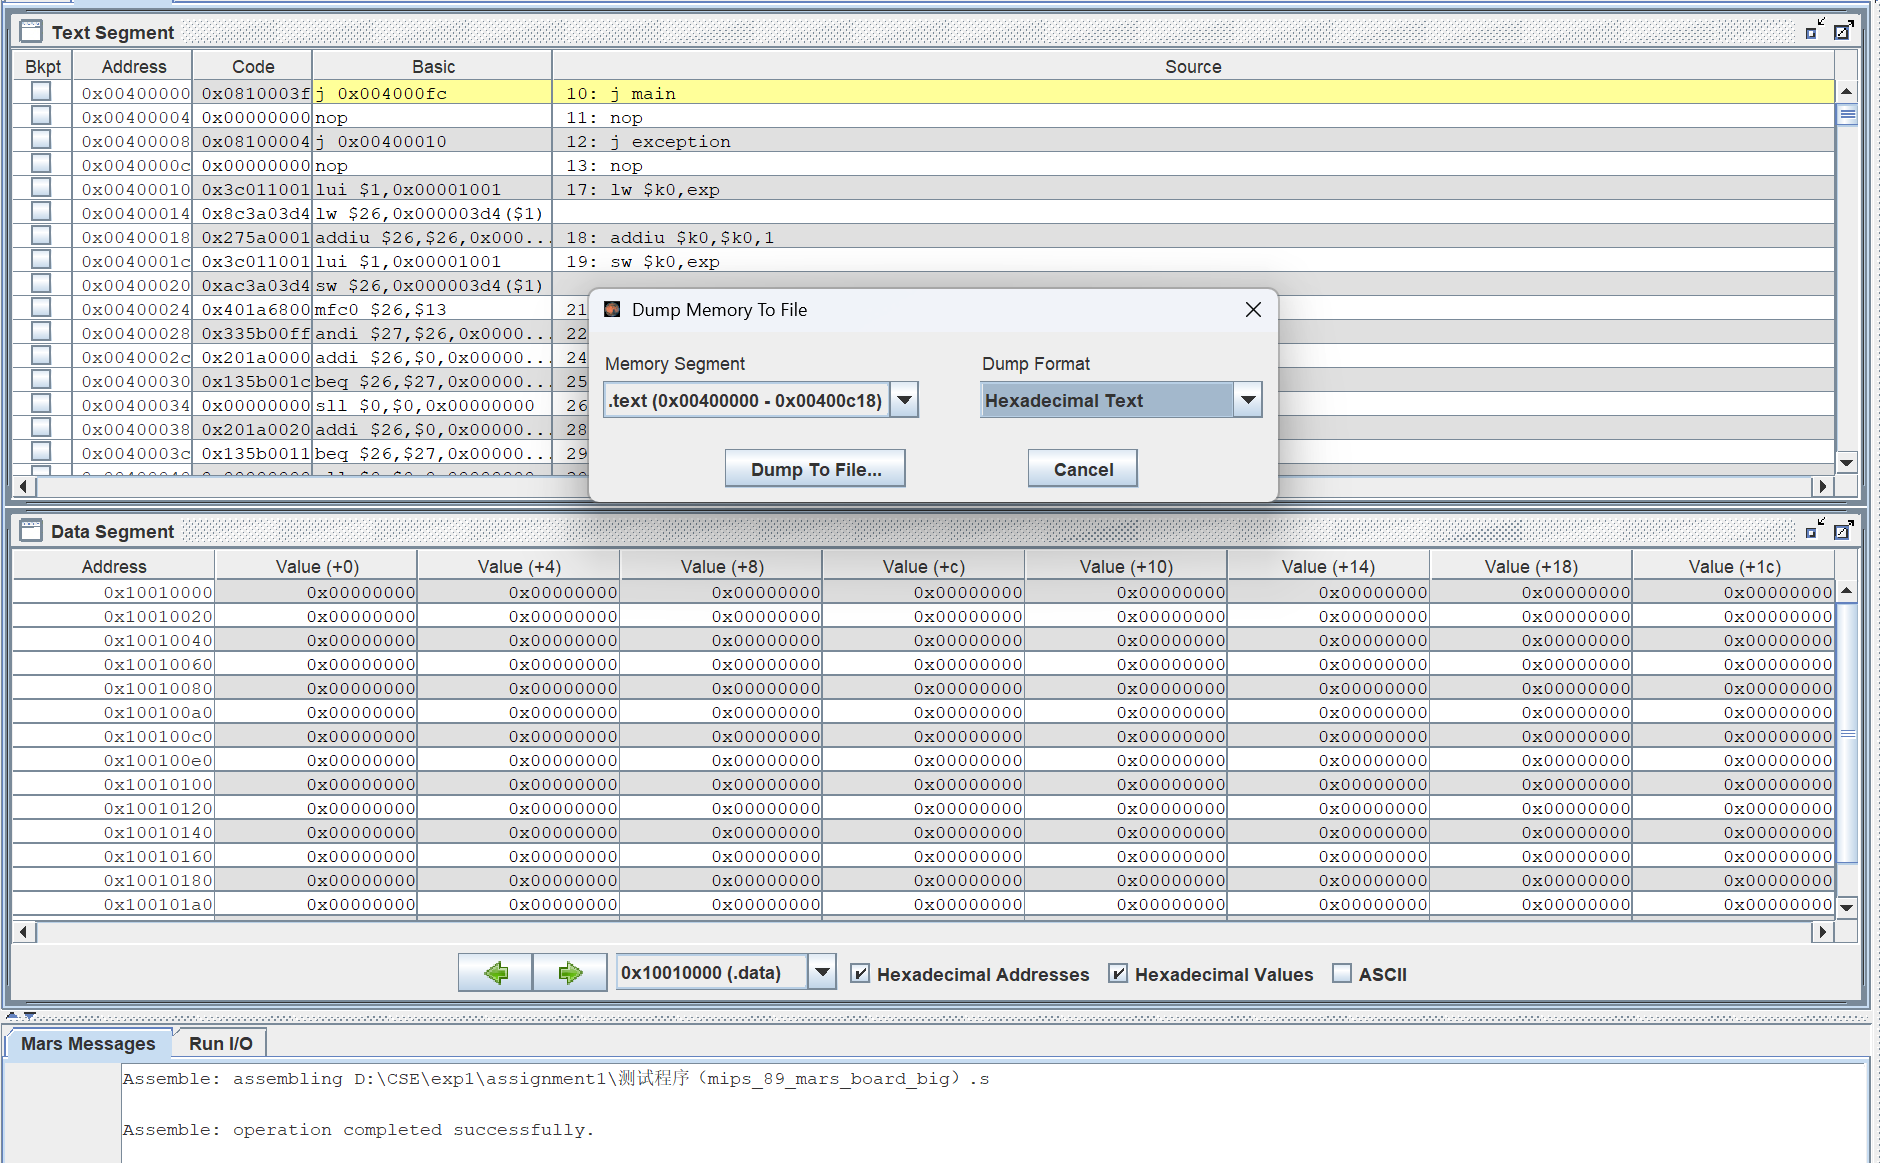
\includegraphics[width=0.8\textwidth]{img/mars_export.png}
    \caption{MARS汇编器导出机器码}
\end{figure}

IP核配置参数：
\begin{itemize}[leftmargin=2em]
    \item 名称：\texttt{inst\_rom\_for\_cpu89}
    \item 深度：2048
    \item 数据宽度：32位
    \item 类型：ROM
    \item 输入/输出选项：Non Registered
\end{itemize}

\begin{figure}[H]
    \centering
    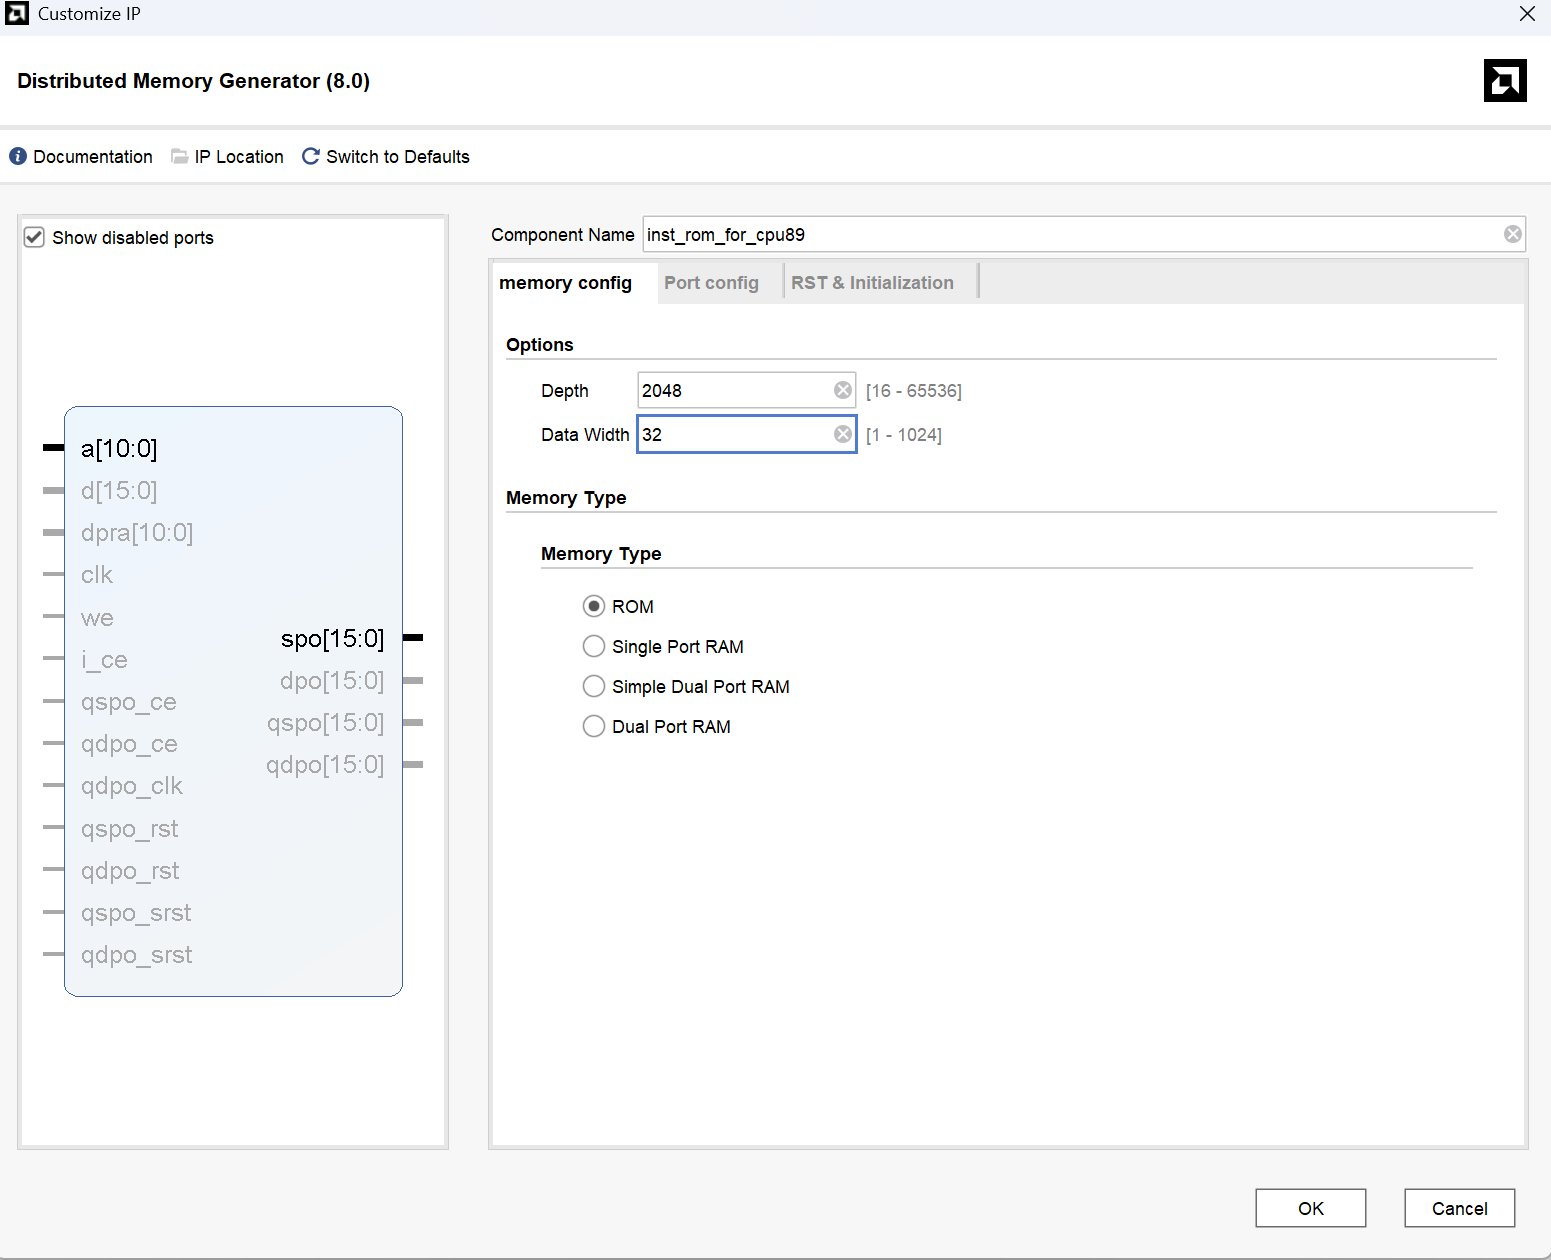
\includegraphics[width=0.8\textwidth]{img/ip_core_generate.png}
    \caption{Distributed Memory Generator IP核生成}
\end{figure}

\subsection{引脚分配}

\begin{table}[H]
    \centering
    \caption{FPGA引脚分配}
    \begin{tabular}{lll}
        \toprule
        \textbf{信号} & \textbf{引脚} & \textbf{功能说明} \\
        \midrule
        \texttt{clk\_in} & E3 & 100MHz板载时钟输入 \\
        \texttt{reset} & N17 & 复位按钮（BTNC） \\
        \texttt{en\_clk} & V10 & 时钟模式选择开关 \\
        \texttt{choose[0]} & J15 & 显示选择开关（低位） \\
        \texttt{choose[1]} & L16 & 显示选择开关（高位） \\
        \texttt{o\_seg[7:0]} & T10,R10,K16,K13,P15,T11,L18,H15 & 七段数码管段选 \\
        \texttt{o\_sel[7:0]} & J17,J18,T9,J14,P14,T14,K2,U13 & 七段数码管位选 \\
        \bottomrule
    \end{tabular}
\end{table}

所有I/O引脚电平标准设置为 LVCMOS33。

\subsection{综合与实现}

\begin{enumerate}[leftmargin=2em]
    \item \textbf{综合（Synthesis）}：将Verilog代码转换为门级网表。
    \item \textbf{实现（Implementation）}：完成布局布线，将逻辑映射到FPGA具体资源。
    \item \textbf{生成比特流（Generate Bitstream）}：生成可下载到FPGA的配置文件。
\end{enumerate}



\section{Vivado仿真验证}

\subsection{仿真环境配置}

% TODO: 描述仿真testbench的设置，包括时钟周期、复位信号等

使用Vivado自带的仿真工具（Vivado Simulator）对CPU设计进行功能仿真。仿真顶层模块为 \texttt{openmips\_min\_sopc\_tb}，主要配置如下：

\begin{itemize}[leftmargin=2em]
    \item 仿真时钟周期：20ns（50MHz）
    \item 复位信号：仿真开始时拉高，经过若干个时钟周期后释放
    \item 仿真时长：根据测试程序执行所需周期数设定
\end{itemize}

\subsection{仿真波形分析}

% TODO: 插入Vivado仿真波形截图，并对关键信号进行分析

\begin{figure}[H]
    \centering
    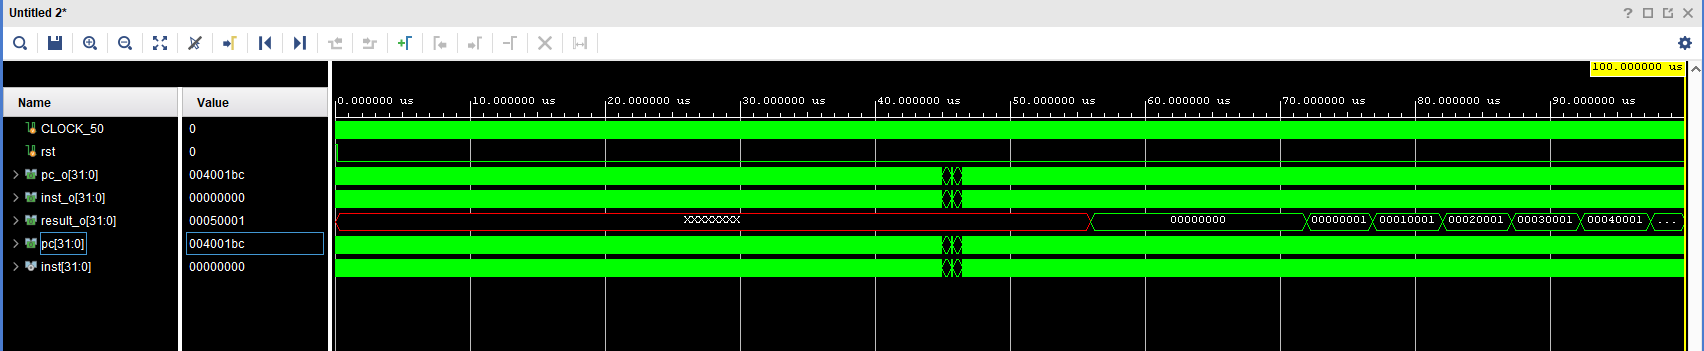
\includegraphics[width=0.9\textwidth]{img/sim_waveform1.png} 
    \caption{仿真波形——整体执行过程}
\end{figure}


\subsection{仿真结果}



\section{实验结果}

\subsection{板级验证结果}

将生成的比特流文件下载到Nexys DDR开发板后，进行以下验证：

\begin{enumerate}[leftmargin=2em]
    \item 将 \texttt{choose} 开关拨至 \texttt{00}（显示数据存储器结果）。
    \item 按下复位按钮后释放，CPU开始执行测试程序。
    \item 观察数码管显示。
\end{enumerate}

\textbf{预期结果}：

\begin{itemize}[leftmargin=2em]
    \item 数码管低半字（低4位数码管）显示 \texttt{0001}，表示全部11个测试函数通过。
    \item 数码管高半字（高4位数码管）持续递增，表示时钟中断功能正常。
\end{itemize}

\textbf{实际验证}：


\begin{figure}[H]
    \centering
    % TODO: 替换为数码管显示0001的开发板实物照片
    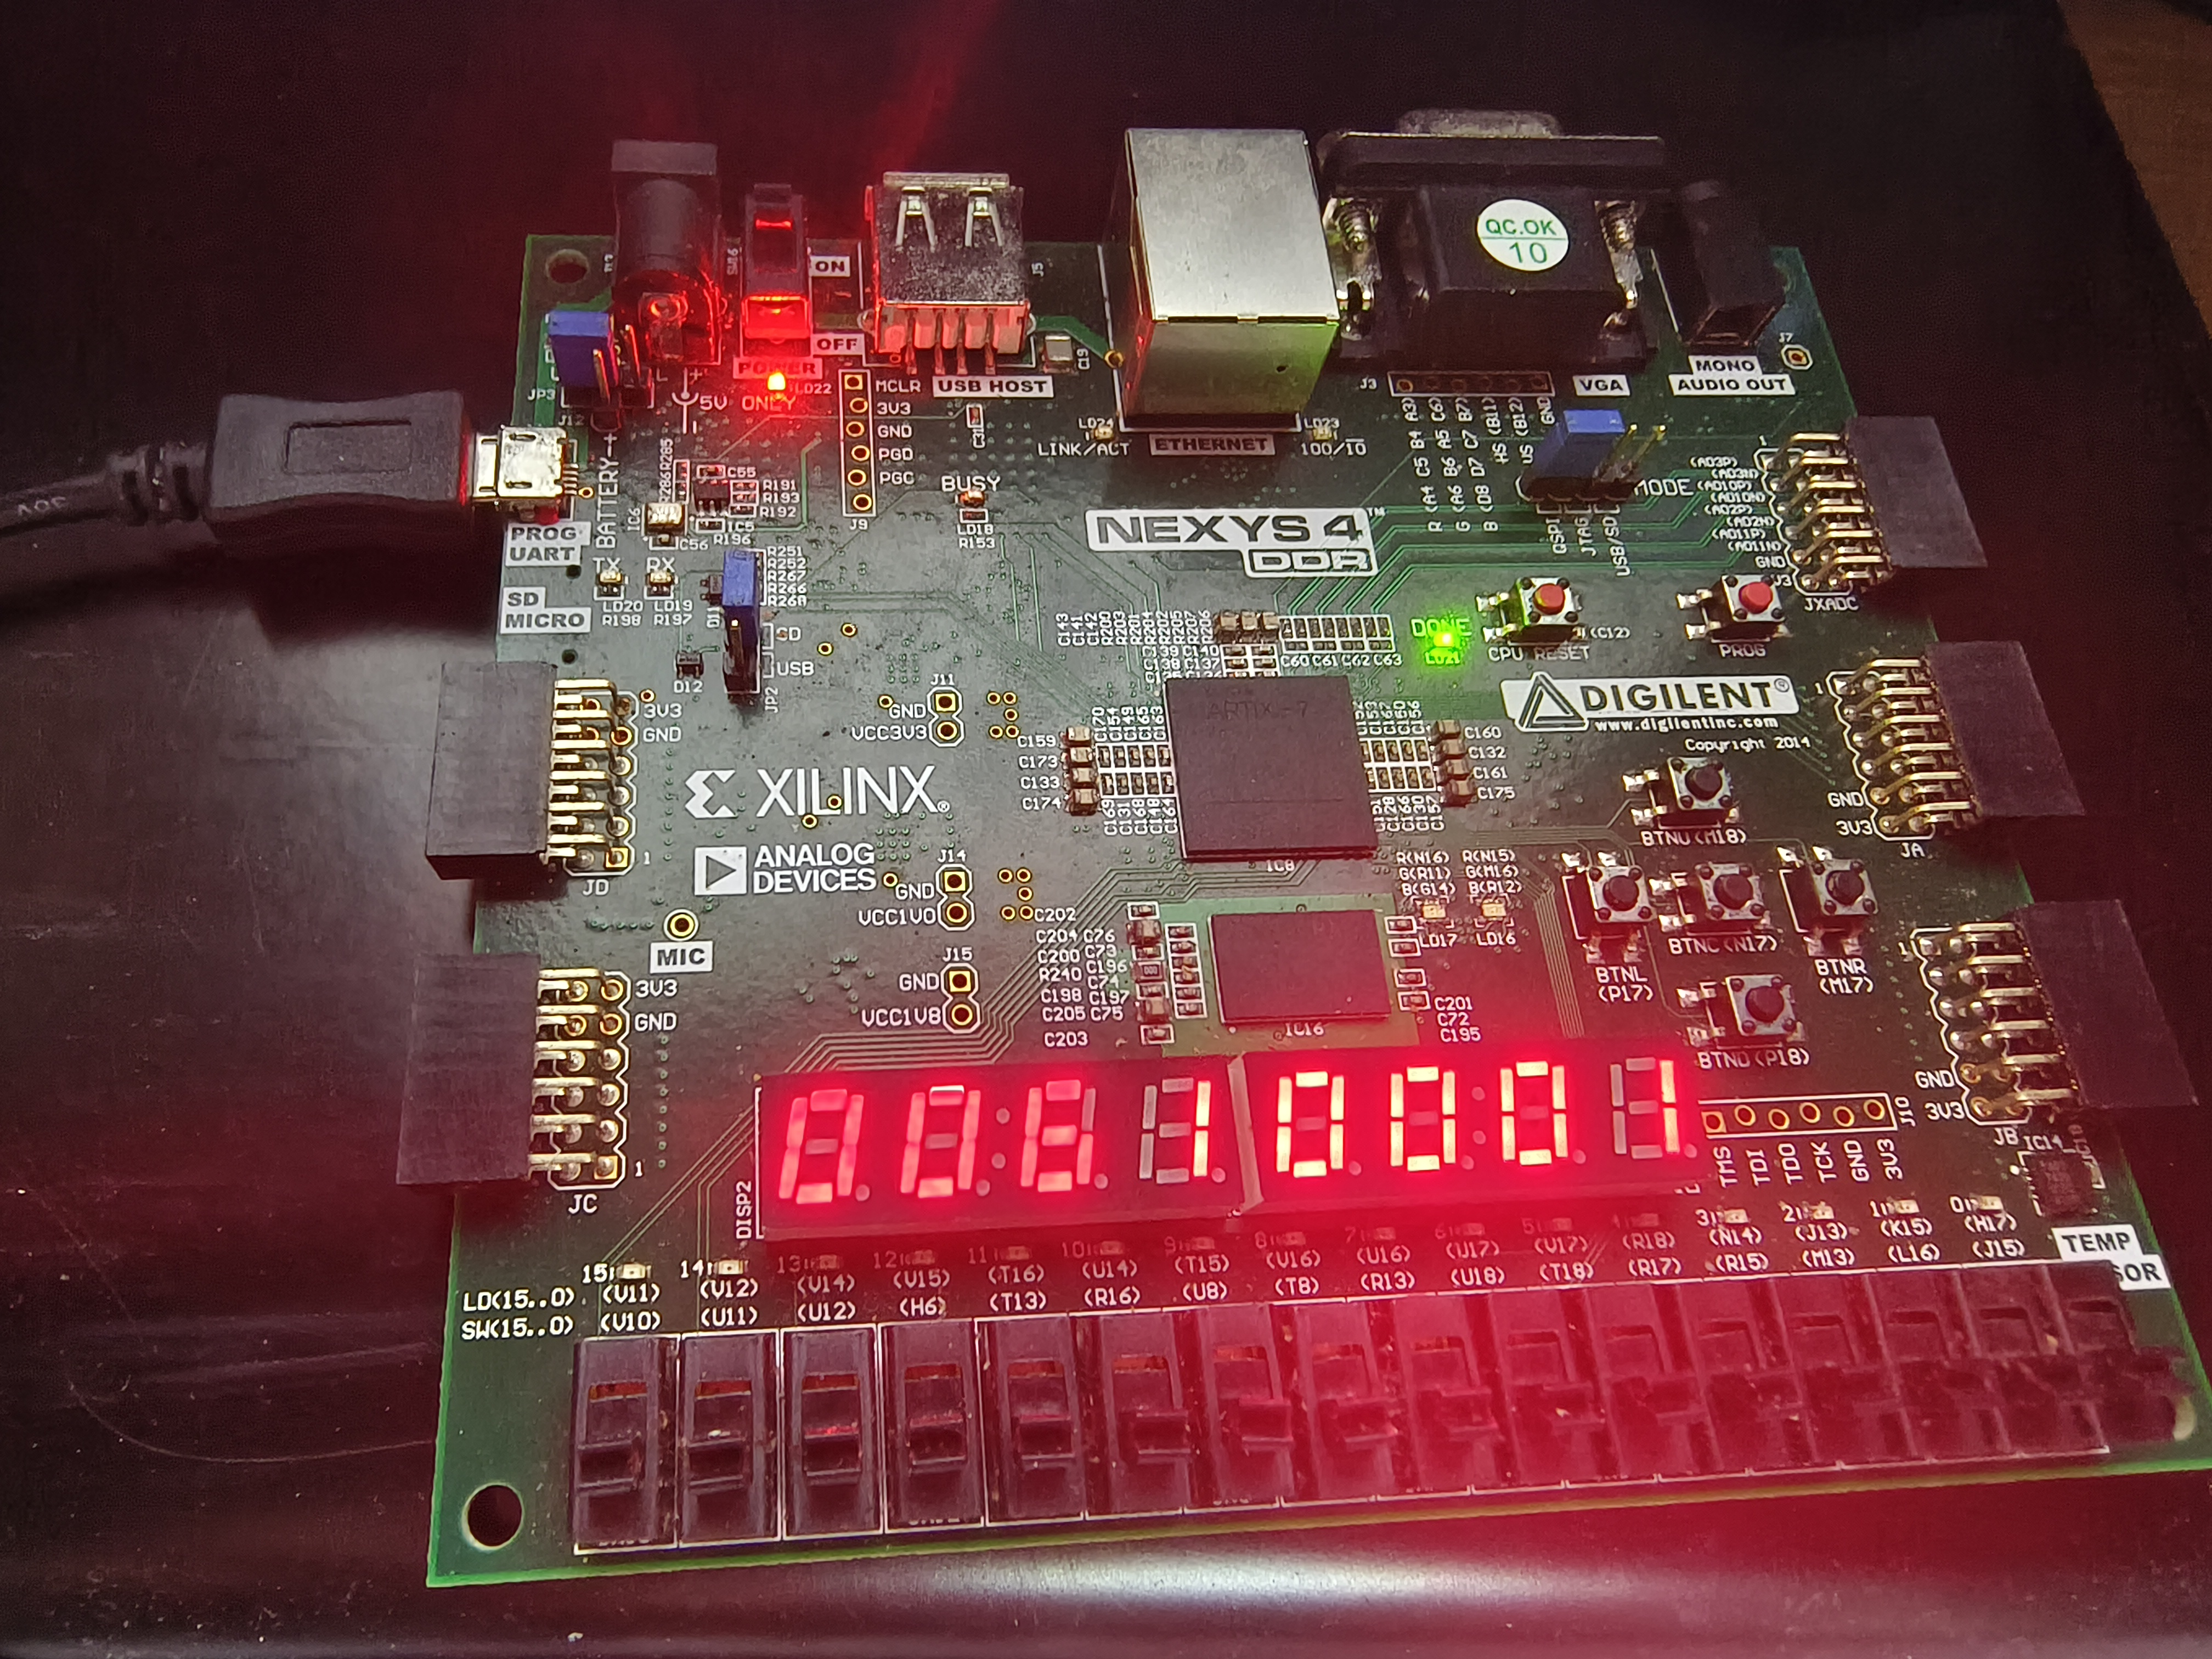
\includegraphics[width=0.6\textwidth]{img/board_result1.jpg}
    \caption{测试通过——数码管低半字显示0001}
\end{figure}

\begin{figure}[H]
    \centering
    % TODO: 替换为数码管高半字递增的开发板实物照片
    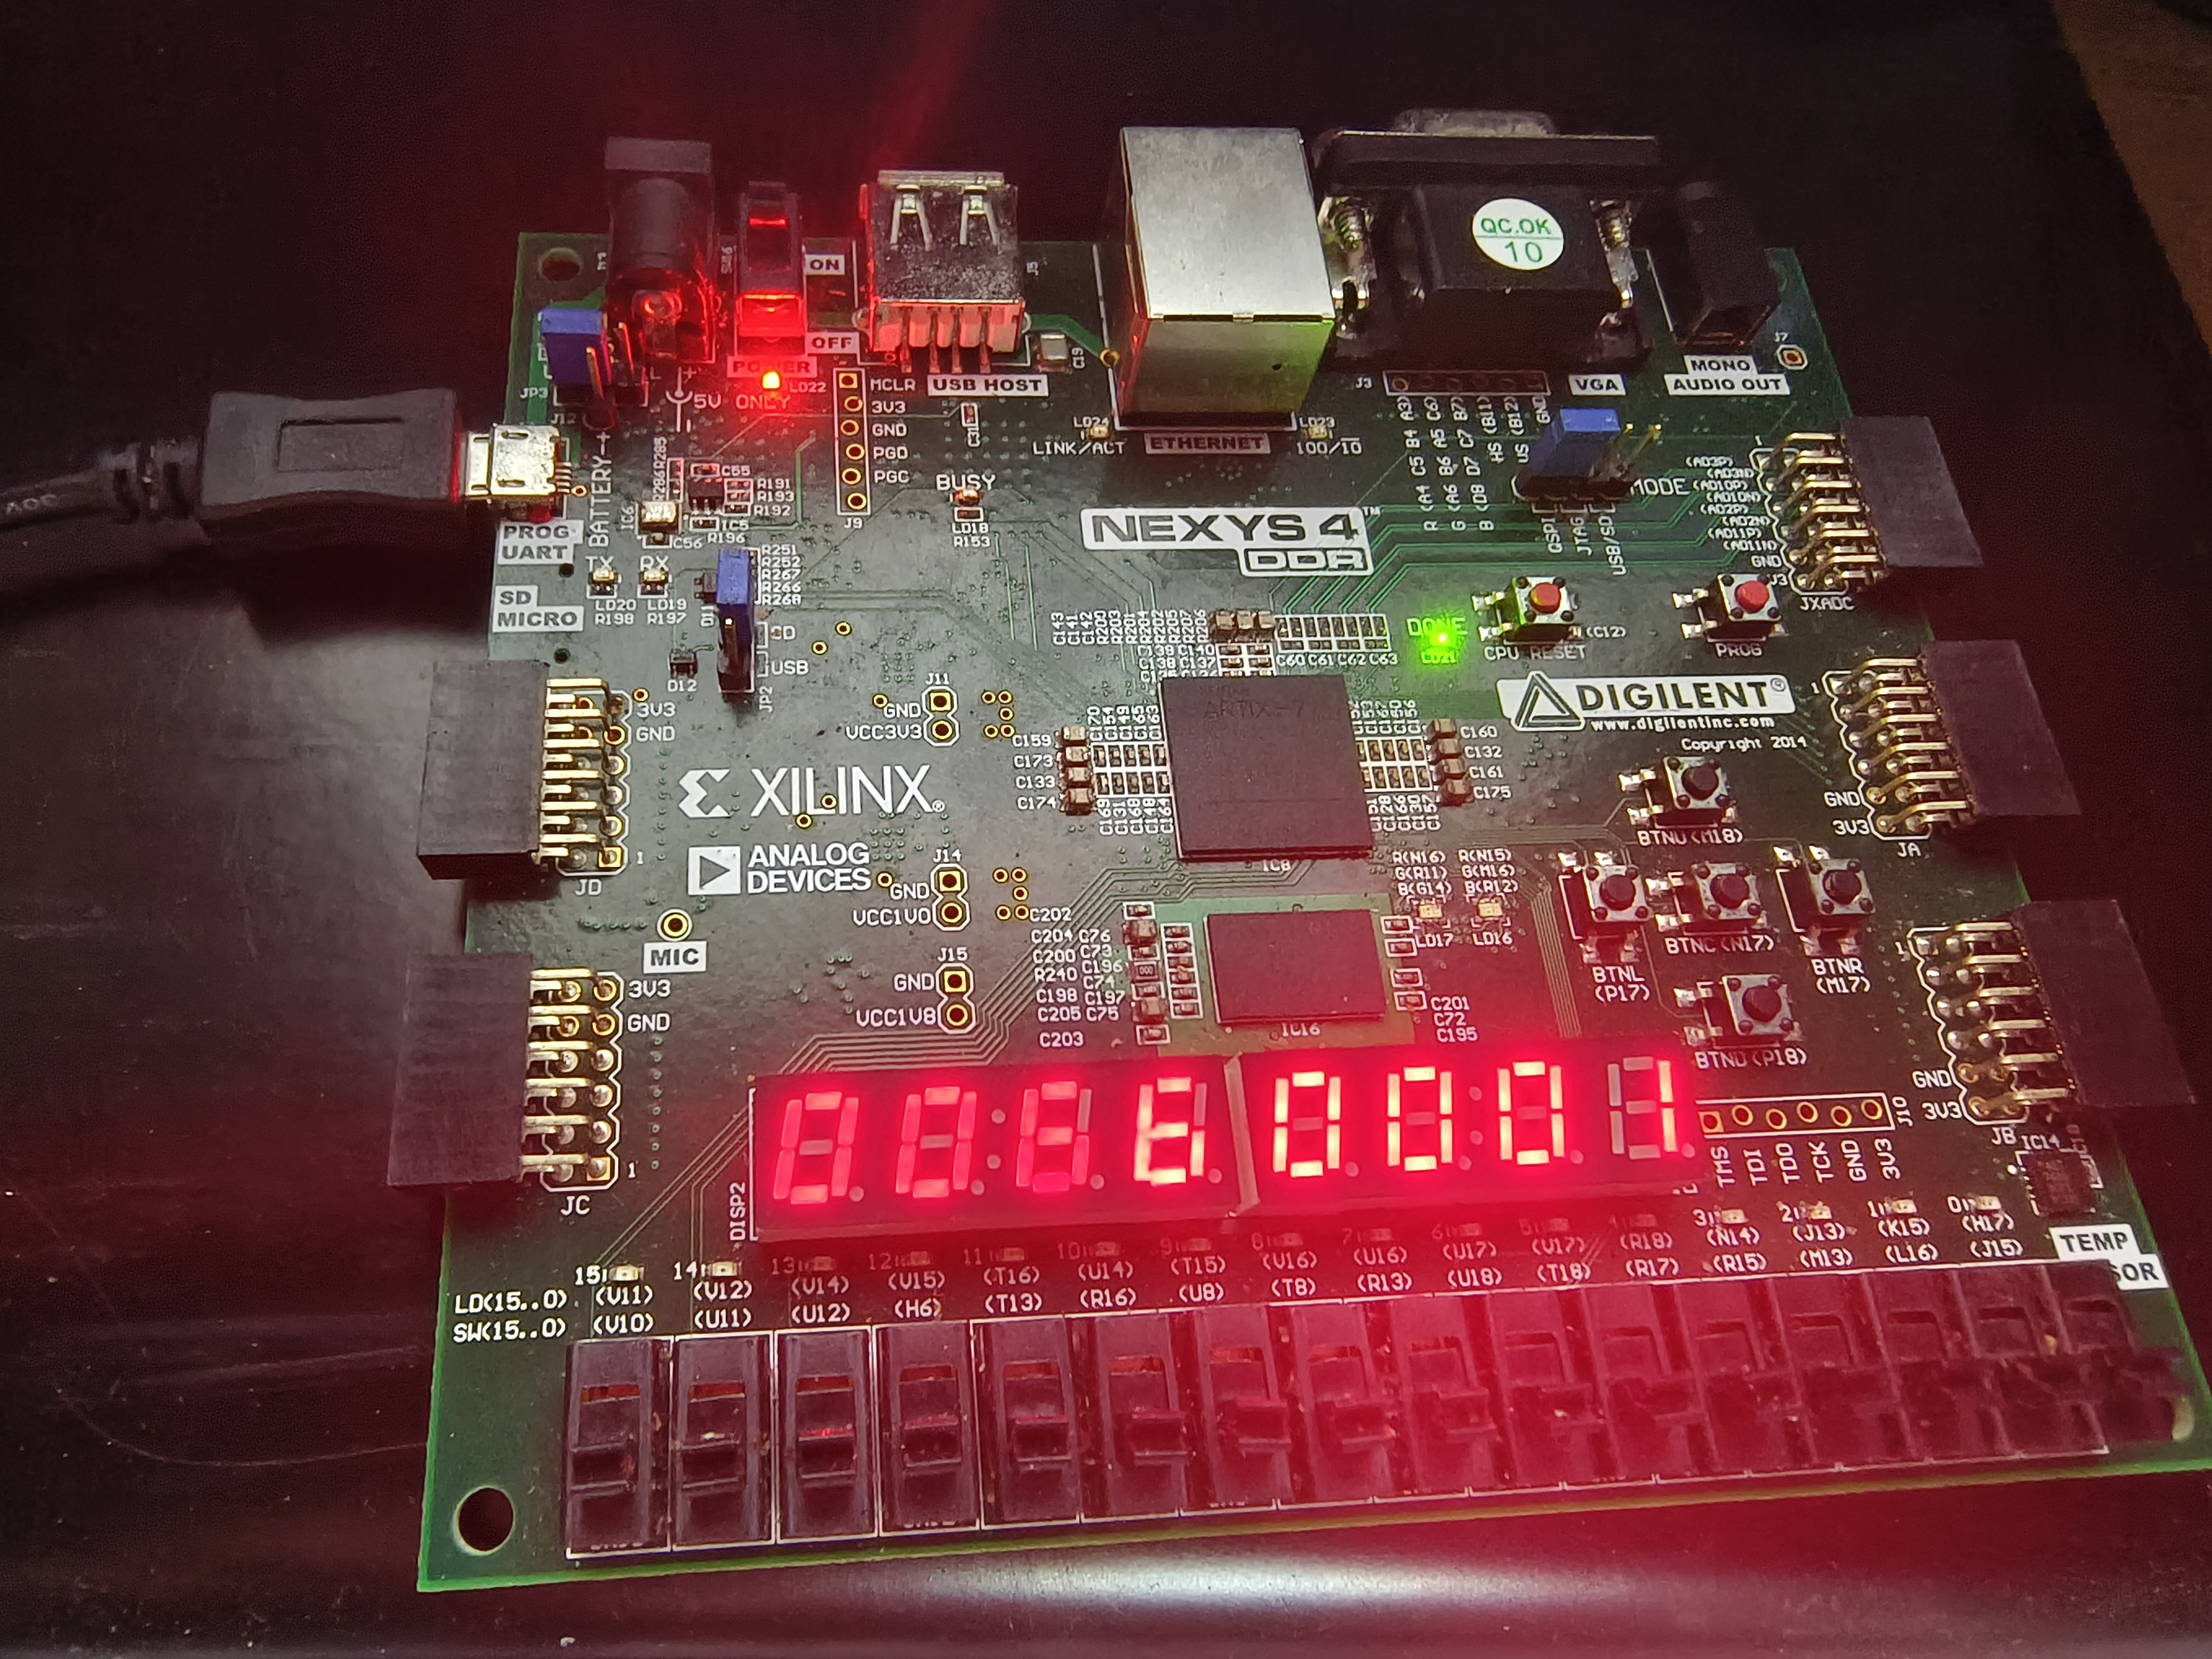
\includegraphics[width=0.6\textwidth]{img/board_result2.jpg}
    \caption{时钟中断正常——数码管高半字持续递增}
\end{figure}

\section{实验总结}

\subsection{实验收获}

通过本次CPU改造实验，我对以下内容有了更深入的理解：

\begin{enumerate}[leftmargin=2em]
    \item \textbf{MIPS指令集架构}：掌握了89条MIPS指令的编码格式、语义和流水线执行过程，理解了R型、I型、J型三种指令格式的设计原理。

    \item \textbf{五级流水线设计}：深入理解了取指、译码、执行、访存、写回五个阶段的划分依据，以及各阶段之间通过流水线寄存器传递数据的机制。

    \item \textbf{冒险处理}：掌握了数据前推（forwarding）解决数据冒险的方法，理解了load-use冒险必须插入气泡的原因，以及控制冒险通过延迟槽处理的机制。

    \item \textbf{异常与中断}：理解了精确异常模型的实现方式——异常在流水线末端（MEM阶段）统一判定，通过flush信号清空流水线，保证异常指令之前的指令全部完成、之后的指令全部取消。

    \item \textbf{CP0协处理器}：掌握了Status、Cause、EPC等关键寄存器的功能和交互方式，理解了时钟中断从触发到响应再到返回的完整流程。

    \item \textbf{FPGA开发流程}：熟悉了Vivado工具链从创建工程、添加源文件、创建IP核、综合实现到下载验证的完整流程。
\end{enumerate}

\subsection{遇到的问题与解决方法}

\begin{enumerate}[leftmargin=2em]
    \item \textbf{问题}：MARS导出机器码时，需要将汇编程序转换为Vivado IP核可识别的COE格式，但MARS默认导出的是十六进制文本文件，无法直接作为COE文件使用。\\
          \textbf{解决}：在MARS中选择 File $\rightarrow$ Dump Memory，导出格式选择"Binary Text"，得到每行一条32位二进制指令的文本文件。随后编写脚本在文件头部添加 \texttt{memory\_initialization\_radix=2;} 和 \texttt{memory\_initialization\_vector=} 头信息，每行末尾添加逗号分隔符，将其转换为标准COE格式，成功用于Distributed Memory Generator IP核的初始化。

    \item \textbf{问题}：Vivado综合阶段报告关键路径时序违规（Timing Not Met），提示 \texttt{WNS}（Worst Negative Slack）为负值，涉及的路径主要在除法器的32轮迭代逻辑和多级数据前推的组合逻辑链上。\\
          \textbf{解决}：分析发现时序约束是针对板载100MHz时钟（10ns周期）设定的，而实际CPU工作时钟经过 \texttt{divider}模块100000倍分频后频率远低于1kHz，组合逻辑延迟在实际工作频率下完全满足要求。因此该时序违规警告不影响实际功能，可安全忽略。

\end{enumerate}



\end{document}
